
\documentclass[11pt,compress,t,notes=noshow, xcolor=table]{beamer}
\usepackage[]{graphicx}\usepackage[]{color}
% maxwidth is the original width if it is less than linewidth
% otherwise use linewidth (to make sure the graphics do not exceed the margin)
\makeatletter
\def\maxwidth{ %
  \ifdim\Gin@nat@width>\linewidth
    \linewidth
  \else
    \Gin@nat@width
  \fi
}
\makeatother

\definecolor{fgcolor}{rgb}{0.345, 0.345, 0.345}
\newcommand{\hlnum}[1]{\textcolor[rgb]{0.686,0.059,0.569}{#1}}%
\newcommand{\hlstr}[1]{\textcolor[rgb]{0.192,0.494,0.8}{#1}}%
\newcommand{\hlcom}[1]{\textcolor[rgb]{0.678,0.584,0.686}{\textit{#1}}}%
\newcommand{\hlopt}[1]{\textcolor[rgb]{0,0,0}{#1}}%
\newcommand{\hlstd}[1]{\textcolor[rgb]{0.345,0.345,0.345}{#1}}%
\newcommand{\hlkwa}[1]{\textcolor[rgb]{0.161,0.373,0.58}{\textbf{#1}}}%
\newcommand{\hlkwb}[1]{\textcolor[rgb]{0.69,0.353,0.396}{#1}}%
\newcommand{\hlkwc}[1]{\textcolor[rgb]{0.333,0.667,0.333}{#1}}%
\newcommand{\hlkwd}[1]{\textcolor[rgb]{0.737,0.353,0.396}{\textbf{#1}}}%
\let\hlipl\hlkwb

\usepackage{framed}
\makeatletter
\newenvironment{kframe}{%
 \def\at@end@of@kframe{}%
 \ifinner\ifhmode%
  \def\at@end@of@kframe{\end{minipage}}%
  \begin{minipage}{\columnwidth}%
 \fi\fi%
 \def\FrameCommand##1{\hskip\@totalleftmargin \hskip-\fboxsep
 \colorbox{shadecolor}{##1}\hskip-\fboxsep
     % There is no \\@totalrightmargin, so:
     \hskip-\linewidth \hskip-\@totalleftmargin \hskip\columnwidth}%
 \MakeFramed {\advance\hsize-\width
   \@totalleftmargin\z@ \linewidth\hsize
   \@setminipage}}%
 {\par\unskip\endMakeFramed%
 \at@end@of@kframe}
\makeatother

\definecolor{shadecolor}{rgb}{.97, .97, .97}
\definecolor{messagecolor}{rgb}{0, 0, 0}
\definecolor{warningcolor}{rgb}{1, 0, 1}
\definecolor{errorcolor}{rgb}{1, 0, 0}
\newenvironment{knitrout}{}{} % an empty environment to be redefined in TeX

\usepackage{alltt}
\newcommand{\SweaveOpts}[1]{}  % do not interfere with LaTeX
\newcommand{\SweaveInput}[1]{} % because they are not real TeX commands
\newcommand{\Sexpr}[1]{}       % will only be parsed by R
\newcommand{\xmark}{\ding{55}}%


\usepackage[english]{babel}
\usepackage[utf8]{inputenc}

\usepackage{dsfont}
\usepackage{verbatim}
\usepackage{amsmath}
\usepackage{amsfonts}
\usepackage{amssymb}
\usepackage{bm}
\usepackage{csquotes}
\usepackage{multirow}
\usepackage{longtable}
\usepackage{booktabs}
\usepackage{enumerate}
\usepackage[absolute,overlay]{textpos}
\usepackage{psfrag}
\usepackage{algorithm}
\usepackage{algpseudocode}
\usepackage{eqnarray}
\usepackage{arydshln}
\usepackage{tabularx}
\usepackage{placeins}
\usepackage{tikz}
\usepackage{setspace}
\usepackage{colortbl}
\usepackage{mathtools}
\usepackage{wrapfig}
\usepackage{bm}
\usepackage{amsmath}
\usepackage{pifont}
\usepackage{xcolor} %colored math symbols

\usetikzlibrary{shapes,arrows,automata,positioning,calc,chains,trees, shadows}
\tikzset{
  %Define standard arrow tip
  >=stealth',
  %Define style for boxes
  punkt/.style={
    rectangle,
    rounded corners,
    draw=black, very thick,
    text width=6.5em,
    minimum height=2em,
    text centered},
  % Define arrow style
  pil/.style={
    ->,
    thick,
    shorten <=2pt,
    shorten >=2pt,}
}

\usepackage{subfig}

% Defines macros and environments
\usepackage{../../style/lmu-lecture}


\let\code=\texttt
\let\proglang=\textsf

\setkeys{Gin}{width=0.9\textwidth}

\setbeamertemplate{frametitle}{\expandafter\uppercase\expandafter\insertframetitle}

\usepackage{bbm}
% basic latex stuff
\newcommand{\pkg}[1]{{\fontseries{b}\selectfont #1}} %fontstyle for R packages
\newcommand{\lz}{\vspace{0.5cm}} %vertical space
\newcommand{\dlz}{\vspace{1cm}} %double vertical space
\newcommand{\oneliner}[1] % Oneliner for important statements
{\begin{block}{}\begin{center}\begin{Large}#1\end{Large}\end{center}\end{block}}


%new environments
\newenvironment{vbframe}  %frame with breaks and verbatim
{
 \begin{frame}[containsverbatim,allowframebreaks]
}
{
\end{frame}
}

\newenvironment{vframe}  %frame with verbatim without breaks (to avoid numbering one slided frames)
{
 \begin{frame}[containsverbatim]
}
{
\end{frame}
}

\newenvironment{blocki}[1]   % itemize block
{
 \begin{block}{#1}\begin{itemize}
}
{
\end{itemize}\end{block}
}

\newenvironment{fragileframe}[2]{  %fragile frame with framebreaks
\begin{frame}[allowframebreaks, fragile, environment = fragileframe]
\frametitle{#1}
#2}
{\end{frame}}


\newcommand{\myframe}[2]{  %short for frame with framebreaks
\begin{frame}[allowframebreaks]
\frametitle{#1}
#2
\end{frame}}

\newcommand{\remark}[1]{
  \textbf{Remark:} #1
}


\newenvironment{deleteframe}
{
\begingroup
\usebackgroundtemplate{
\includegraphics[width=\paperwidth,height=\paperheight]{../style/color/red.png}}
 \begin{frame}
}
{
\end{frame}
\endgroup
}
\newenvironment{simplifyframe}
{
\begingroup
\usebackgroundtemplate{
\includegraphics[width=\paperwidth,height=\paperheight]{../style/color/yellow.png}}
 \begin{frame}
}
{
\end{frame}
\endgroup
}\newenvironment{draftframe}
{
\begingroup
\usebackgroundtemplate{
\includegraphics[width=\paperwidth,height=\paperheight]{../style/color/green.jpg}}
 \begin{frame}
}
{
\end{frame}
\endgroup
}
% https://tex.stackexchange.com/a/261480: textcolor that works in mathmode
\makeatletter
\renewcommand*{\@textcolor}[3]{%
  \protect\leavevmode
  \begingroup
    \color#1{#2}#3%
  \endgroup
}
\makeatother


\input{../../latex-math/basic-math}
\input{../../latex-math/basic-ml}
\input{../../latex-math/ml-nn}

\newcommand{\titlefigure}{plots/05_conv_variations/3d/3dconv.png}
%modify picture
\newcommand{\learninggoals}{
  \item 1D Convolutions
  \item 2D Convolutions
  \item 3D Convolutions
}

\title{Deep Learning}
\date{}



\begin{document}

\lecturechapter{1D / 2D / 3D Convolutions}
\lecture{I2DL}

%%%%%%%%%%%%%%%%%%%%%%%%%%%%%%%%%%%%%%%%%%%%%%%%%%%%%%%%%%%%%%%%%%
%%%%%%%%%%%%%%%%%%%%%%%%%%%%%%%%%%%%%%%%%%%%%%%%%%%%%%%%%%%%%%%%%%


\begin{vbframe}{Famous architectures: LeNet}
  \begin{itemize}
    \item Pioneering work on CNNs by Yann Lecun in 1998. 
    \item Applied on the MNIST dataset for automated handwritten digit recognition.
    \item Consists of convolutional, "subsampling" and dense layers.
    \item Complexity and depth of the net was mainly restricted by limited computational power back in the days.
  \end{itemize}
  \begin{figure}
  \centering
    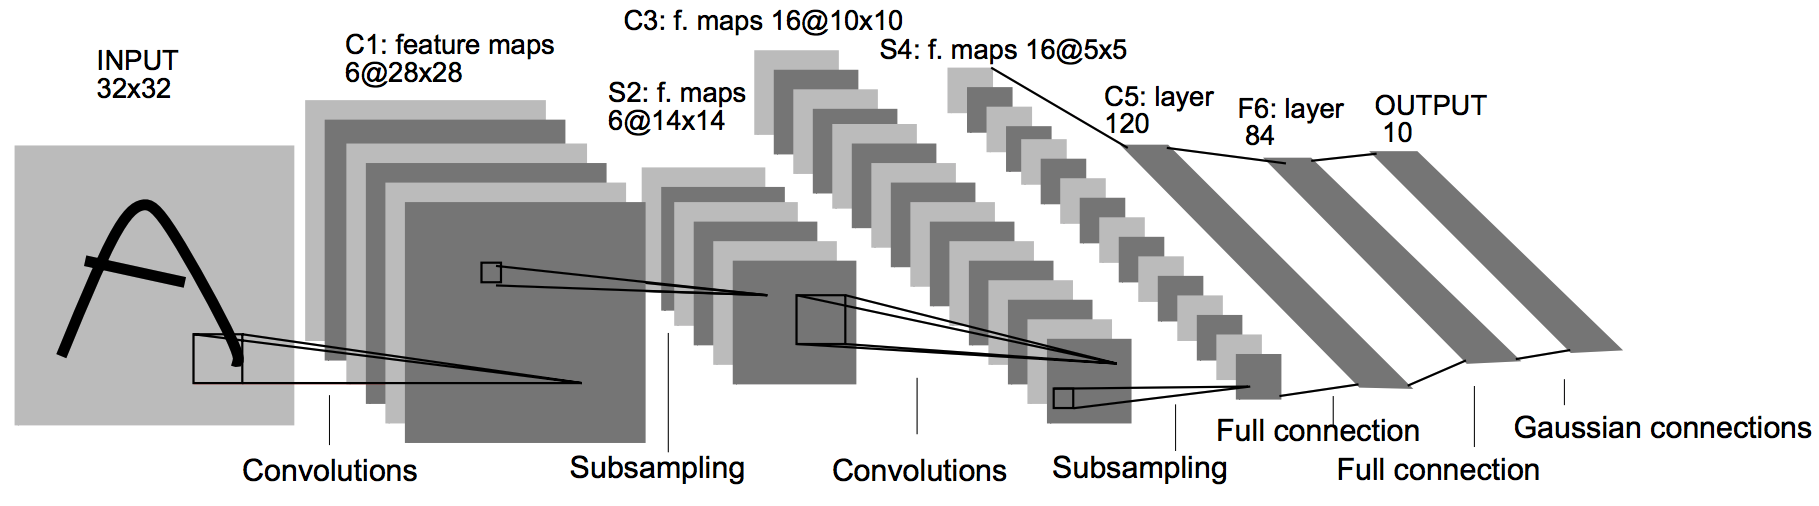
\includegraphics[width=9cm]{plots/architectures/lenet.png}
    \caption{LeNet architecture: two conv layers with subsampling, followed by dense layers and a 'Gaussian connections' layer.}
  \end{figure}
  \framebreak
  
  
  \begin{itemize}
    \item A neuron in a subsampling layer looks at a $2 \times 2$ region of a feature map, sums the four values, multiplies it by a trainable coefficient, adds a trainable bias and then applies a sigmoid activation.
    \item A stride of 2 ensures that the size of the feature map reduces by about a half.
    \item The 'Gaussian connections' layer has a neuron for each possible class. 
    \item The output of each neuron in this layer is the (squared) Euclidean distance between the activations from the previous layer and the weights of the neuron.
  \end{itemize}
\end{vbframe}
%%%%%%%%%%%%%%%%%%%%%%%%%%%%%%%%%%%%%%%%%%%%%%%%%%%%%%%%%%%%%%%%%%
%%%%%%%%%%%%%%%%%%%%%%%%%%%%%%%%%%%%%%%%%%%%%%%%%%%%%%%%%%%%%%%%%%
\begin{vbframe}{Famous architectures: AlexNet}
  \begin{itemize}
    \item Introduced by \textit{Krizhevsky et al., 2012}, won the ImageNet challenge in 2012 and is basically a deeper version of the LeNet.
    \item Trained in parallel on two GPUs, using two streams of convolutions which are partly interconnected.
    \item Contains ReLU activations and makes use of data set augmentation strategies.
  \end{itemize}
  \begin{figure}
  \centering
    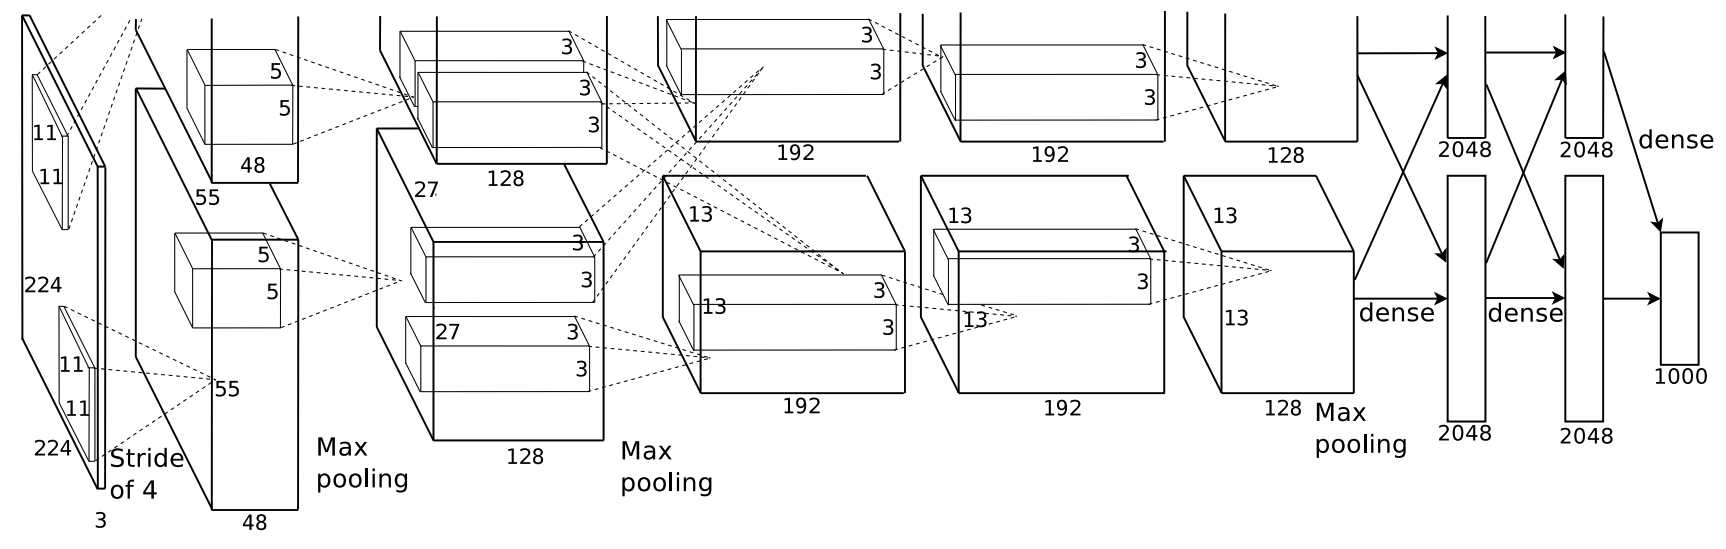
\includegraphics[width=9cm]{plots/architectures/alexnet.png}
    \caption{AlexNet architecture.}
  \end{figure}
\end{vbframe}
%%%%%%%%%%%%%%%%%%%%%%%%%%%%%%%%%%%%%%%%%%%%%%%%%%%%%%%%%%%%%%%%%%
%%%%%%%%%%%%%%%%%%%%%%%%%%%%%%%%%%%%%%%%%%%%%%%%%%%%%%%%%%%%%%%%%%
\begin{vbframe}{Famous architectures: VGG}
  \begin{itemize}
    \item Architecture introduced by \textit{Simoyan et. al, 2014]} as \enquote{Very Deep Convolutional Network}.
    \item A deeper variant of the AlexNet.
    \item Mainly uses many convolutional layers with a small kernel size 3x3.
    \item Performed very well in the ImageNet Challenge 2014.
    \item Exists in a small version (VGG16) with a total of 16 layers and a larger version (VGG19) with 19 layers.
  \end{itemize}
\framebreak
  \begin{figure}
  \centering
    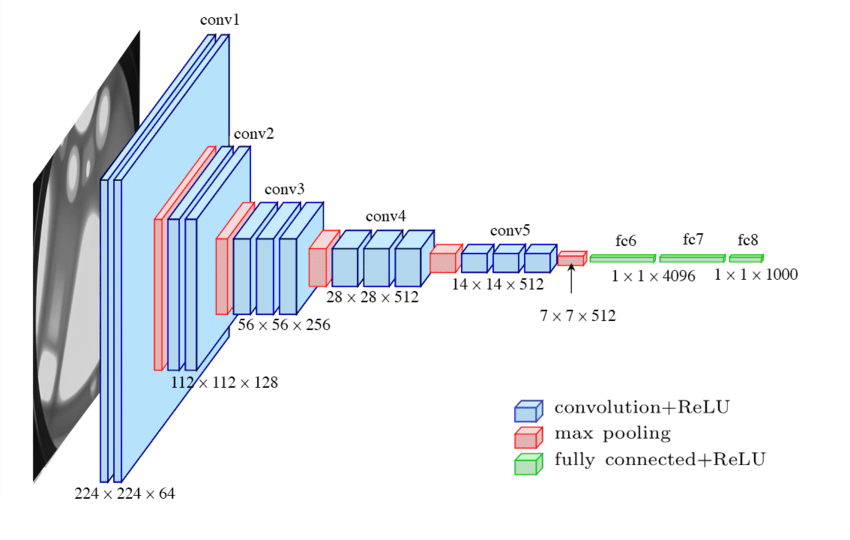
\includegraphics[width=10cm]{plots/architectures/vgg_16n.png}
    \tiny{\\ credit : Max Ferguson}
    \caption{VGG Net 16 with 13 conv layers.}
  \end{figure}
\framebreak
  \begin{figure}
  \centering
    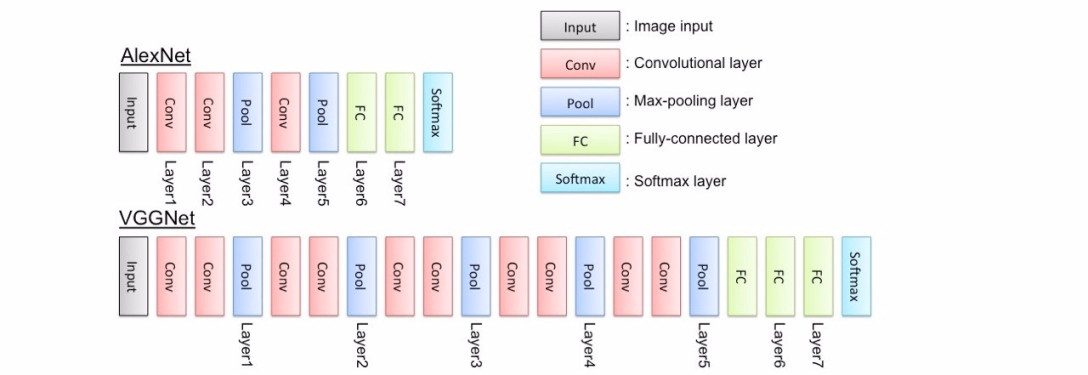
\includegraphics[width=13cm]{plots/architectures/vgg.png}
    \caption{VGG Net with 10 conv layers in comparison with AlexNet.}
  \end{figure}
\end{vbframe}
%%%%%%%%%%%%%%%%%%%%%%%%%%%%%%%%%%%%%%%%%%%%%%%%%%%%%%%%%%%%%%%%%%
%%%%%%%%%%%%%%%%%%%%%%%%%%%%%%%%%%%%%%%%%%%%%%%%%%%%%%%%%%%%%%%%%%
\begin{vbframe}{Famous architectures: GoogLeNet}
  \begin{itemize}
    \item The net architecture that first made use of inception modules.
    \item Also referred to as Inception Net.
    \item Also includes Batch Normalization to improve training.
    \item Uses auxiliary losses: branches throughout the net that consist of softmax layers that make predictions using early stage layers.
    \item Those losses are jointly optimized and the output from the final head is used for deployment and testing of the architecture.
    \item Inception modules allow the net to \enquote{choose} between different kernels.
  \end{itemize}
\framebreak
  \begin{figure}
  \centering
    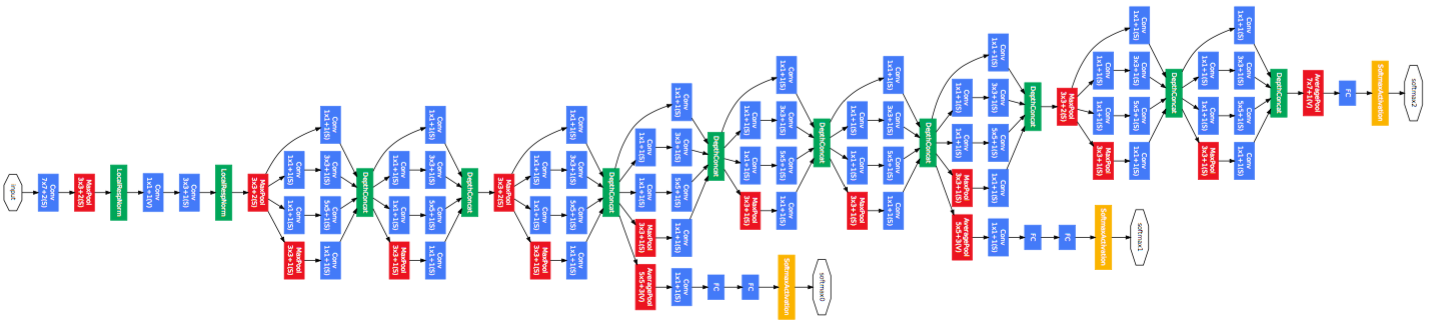
\includegraphics[width=11.5cm]{plots/architectures/googlenet.png}
    \caption{GoogleNet architecture. Yellow rectangles mark the auxiliary losses which are combined during training.}
  \end{figure}
\framebreak
  \begin{figure}
  \centering
    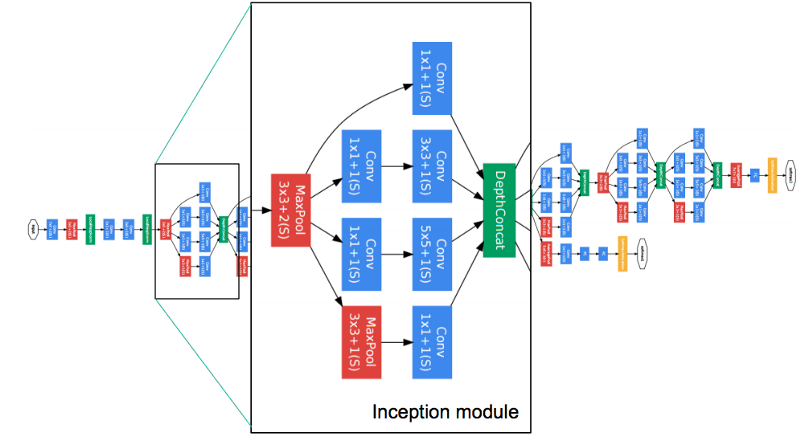
\includegraphics[width=11cm]{plots/05_conv_variations/inception/googlenet.png}
    \caption{Zoom view in one of the inception modules upon which the GoogLeNet architecture is build.}
  \end{figure}
\end{vbframe}
%%%%%%%%%%%%%%%%%%%%%%%%%%%%%%%%%%%%%%%%%%%%%%%%%%%%%%%%%%%%%%%%%%
%%%%%%%%%%%%%%%%%%%%%%%%%%%%%%%%%%%%%%%%%%%%%%%%%%%%%%%%%%%%%%%%%%
\begin{vbframe}{Famous architectures: ResNet}
  \begin{itemize}
    \item Net architecture that makes use of skip connections / residual learning.
    \item This allowed (\textit{He et. al , 2015}) to create a very deep net architectures of up to 152 layers.
    \item Batch normalization and global average pooling is used.
  \end{itemize}
\framebreak
  \begin{figure}
  \centering
    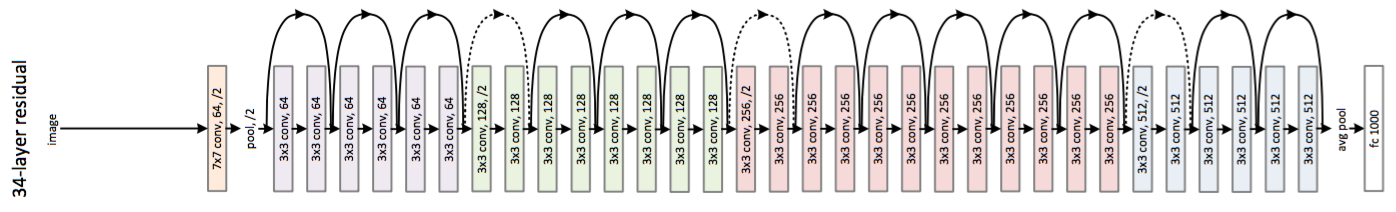
\includegraphics[width=11.5cm]{plots/architectures/resnet.png}
    \caption{A deep ResNet architecture with a total of 34 layers. }
  \end{figure}
\framebreak
  \begin{figure}
  \centering
    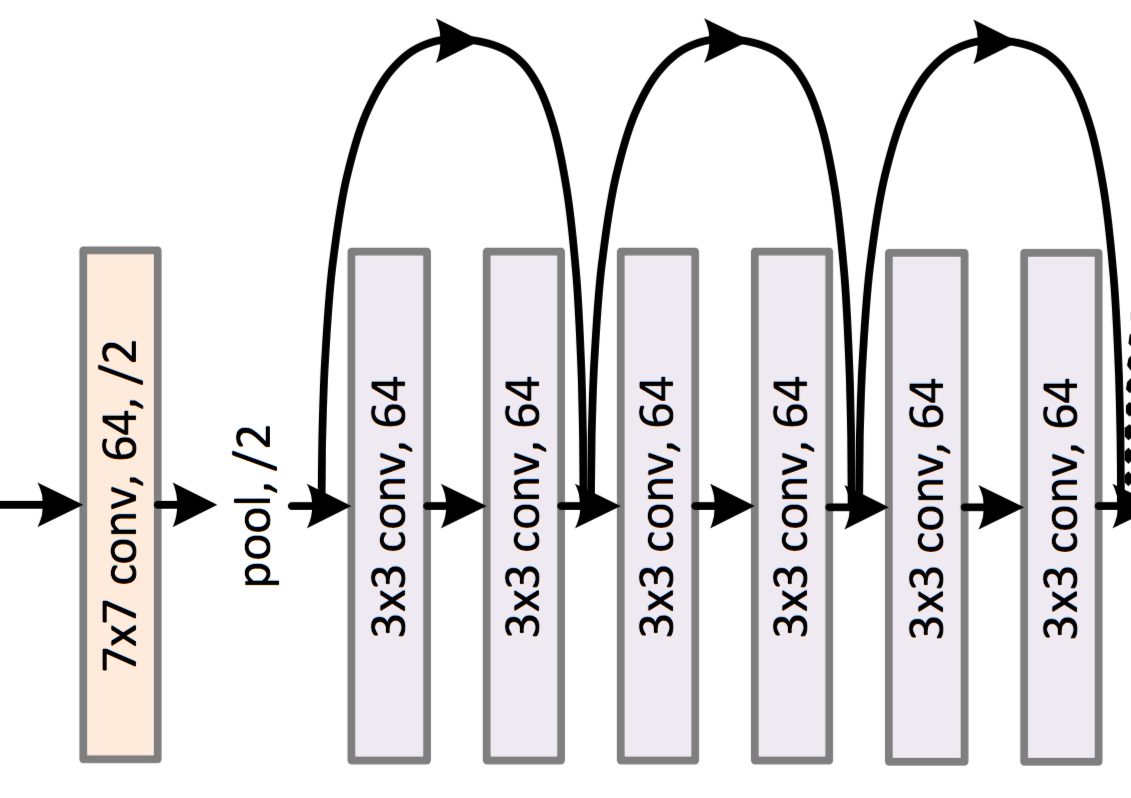
\includegraphics[width=5cm]{plots/architectures/resnet_zoom.png}
    \caption{Zoom view in the ResNet architecture. The arrows mark residual connections which allow the net to \enquote{skip} layers which do not contribute to an improvement in the prediction performance.}
  \end{figure}
\end{vbframe}


\begin{vbframe}{Famous architectures:  U-Net}

      \begin{itemize}
        \item U-Net is a fully convolutional net that makes use of upsampling (via transposed convolutions, for example) as well as skip connections.
        \item Input images are getting convolved and down-sampled in the first half of the architecture.
        \item Then, they are getting upsampled and convolved again in the second half to get back to the input dimension.
%        \item Skip connections throughout the net ensure that high-level features from the start can be combined with low-level features throughout the architecture.
        \item Skip connections throughout the net combine feature maps from earlier layers with those from later layers by concatenating both sets of maps along the depth/channel axis.
        \item Only convolutional and no dense layers are used.
    \end{itemize}
\framebreak
    \begin{figure}
        \centering
        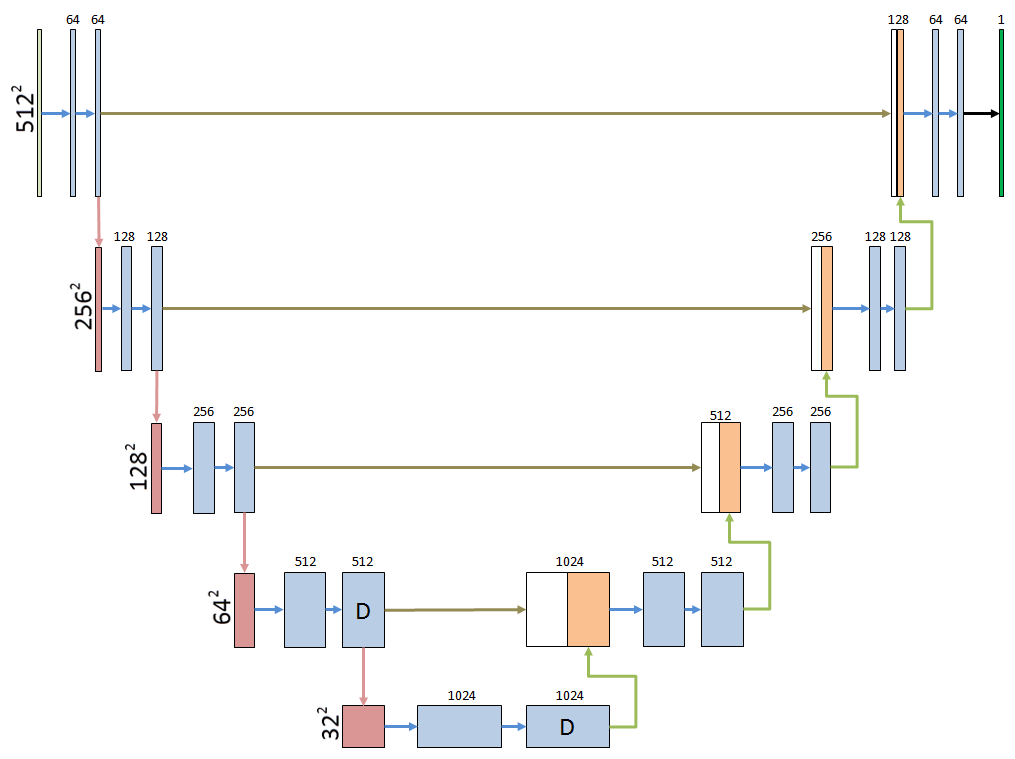
\includegraphics[width=7cm]{plots/outlook/unet.png}
        \caption{Illustration of the architecture. Blue arrows are convolutions, red arrows max-pooling operations, green arrows upsampling steps and the brown arrows merge layers with skip connections. The height and width of the feature blocks are shown on the vertical and the depth on the horizontal. D are dropout layers.}
    \end{figure}
    
\end{vbframe}

\begin{vbframe}{Famous architectures:  U-Net - Example}

    \begin{itemize}
        \item Example problem setting: train a neural net to pixelwise segment roads in satellite imagery.
        \item Answer the question: \textbf{Where is the road map?}
    \end{itemize}
    \begin{figure}
        \centering
        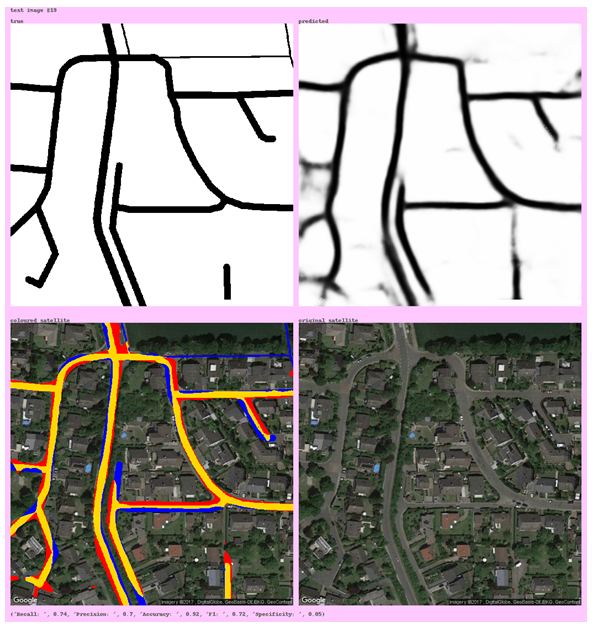
\includegraphics[width=3.8cm]{plots/outlook/31.png}
        \caption{Model prediction on a test satellite image. Yellow are correctly identified pixels, blue false negatives and red false positives.}
    \end{figure}
\framebreak
    \begin{itemize}
        \item The net takes an RGB image [512, 512, 3] and outputs a binary (road / no road) probability mask [512, 512, 1] for each pixel.
        \item The model is trained via a binary cross entropy loss which was combined over each pixel.
    \end{itemize}

  \begin{figure}
        \centering
        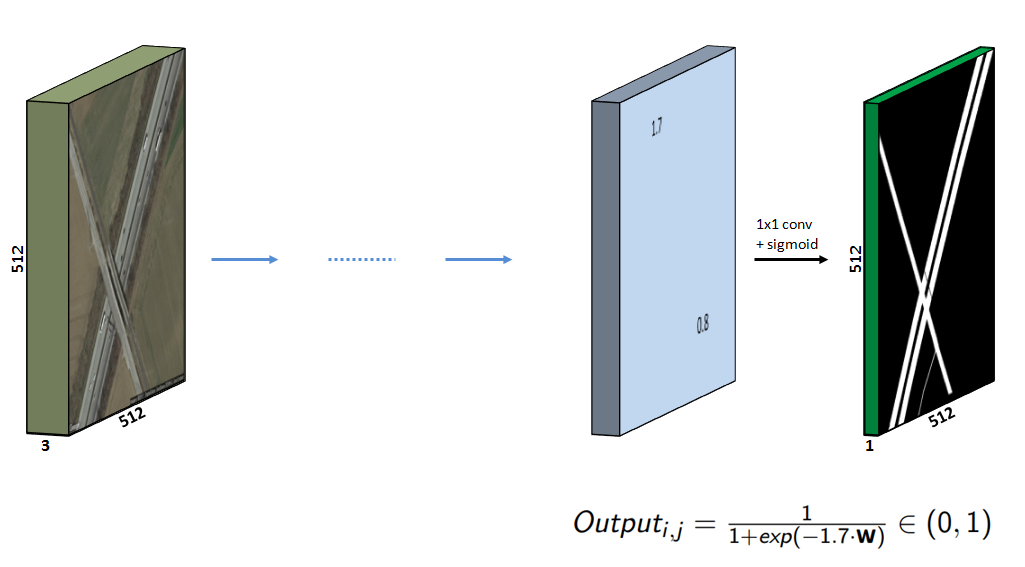
\includegraphics[width=8cm]{plots/outlook/architecture_4.png}
        \caption{Scheme for the input/ output of the net architecture.}
    \end{figure}
    
    

\end{vbframe}



%%%%%%%%%%%%%%%%%%%%%%%%%%%%%%%%%%%%%%%%%%%%%%%%%%%%%%%%%%%%%%%%%%
%%%%%%%%%%%%%%%%%%%%%%%%%%%%%%%%%%%%%%%%%%%%%%%%%%%%%%%%%%%%%%%%%%
\begin{vbframe}{Famous architectures: Summary}
  \begin{itemize}
    \item Main points from the previous architectures:
    \begin{itemize}
        \item LeNet was one of the first successful applications of CNNs.
        \item AlexNet is a deeper version of LeNet.
        \item VGG is a deeper version of AlexNet.
        \item ResNet makes heavy use of skip connections.
        \item GoogLeNet uses inception modules.
        \item Batch normalization is often used in modern architectures.
        \item Global average pooling is also a prominent module in modern architectures.
    \end{itemize}
    \item There exists a great variety of different architectures which perform very well on different tasks.
    \item Almost all of the above described architectures exist in extended versions such as the Inception V1 - V4, deeper and shallower ResNets, ResNets for time series ... it is up to you to discover them all.
  \end{itemize}
\end{vbframe}


%%%%%%%%%%%%%%%%%%%%%%%%%%%%%%%%%%%%%%%%%%%%%%%%%%%%%%%%%%%%%%%%%%
%%%%%%%%%%%%%%%%%%          REFERENCES          %%%%%%%%%%%%%%%%%%
%%%%%%%%%%%%%%%%%%%%%%%%%%%%%%%%%%%%%%%%%%%%%%%%%%%%%%%%%%%%%%%%%%
\begin{vbframe}
\frametitle{References}
\footnotesize{
\begin{thebibliography}{99}
%%%%%%%%%%%%%%%%%%%%%%%%%%%%%%%%%%
\bibitem[Krizhevsky et al., 2012]{11} Alex Krizhevsky, Ilya Sutskever and Geoffrey E. Hinton (2012)
\newblock ImageNet Classification with Deep Convolutional Neural Networks
\newblock \emph{\url{https://papers.nips.cc/paper/4824-imagenet-classification-with-deep-convolutional-neural-networks.pdf}}
%%%%%%%%%%%%%%%%%%%%%%%%%%%%%%%%%%
%%%%%%%%%%%%%%%%%%%%%%%%%%%%%%%%%
\bibitem[Szegedy et. al , 2014]{26} Christian Szegedy, Wei Liu, Yangqing Jia, Pierre Sermanet, Scott Reed, Dragomir Anguelov, Dumitru Erhan, Vincent Vanhoucke and Andrew Rabinovich (2014)
\newblock Going deeper with convolutions
\newblock \emph{\url{https://arxiv.org/abs/1409.4842}}
%%%%%%%%%%%%%%%%%%%%%%%%%%%%%%%%%%
%%%%%%%%%%%%%%%%%%%%%%%%%%%%%%%%%%
\bibitem[He et. al , 2015]{29} Kaiming He, Zhang, Xiangyu, Ren, Shaoqing, and Jian Sun (2015)
\newblock Deep Residual Learning for Image Recognition
\newblock \emph{\url{https://arxiv.org/abs/1512.03385}}
%%%%%%%%%%%%%%%%%%%%%%%%%%%%%%%%%%
%%%%%%%%%%%%%%%%%%%%%%%%%%%%%%%%%%
\bibitem[Le Cun et. al, 1998]{33} LeCunn Yann, Bottou, Leon, Bengio, Yoshua and Patrick Haffner (1998)
\newblock Global training of document processing systems using graph transformer networks
\newblock \emph{\url{http://vision.stanford.edu/cs598_spring07/papers/Lecun98.pdf}}
%%%%%%%%%%%%%%%%%%%%%%%%%%%%%%%%%%
%%%%%%%%%%%%%%%%%%%%%%%%%%%%%%%%%%
\bibitem[Simoyan et. al, 2014]{35} Simoyan Karen and Andrew Zisserman (2014)
\newblock Very Deep Convolutional Networks for Large-Scale Image Recognition
\newblock \emph{\url{https://arxiv.org/abs/1409.1556}}
%%%%%%%%%%%%%%%%%%%%%%%%%%%%%%%%%%
%%%%%%%%%%%%%%%%%%%%%%%%%%%%%%%%%%
\bibitem[Ronneberger et al., 2015]{12} Olaf Ronneberger, Philipp Fischer, Thomas Brox (2015)
\newblock U-Net: Convolutional Networks for Biomedical Image Segmentation
\newblock \emph{\url{http://arxiv.org/abs/1505.04597}}
%%%%%%%%%%%%%%%%%%%%%%%%%%%%%%%%%%
%%%%%%%%%%%%%%%%%%%%%%%%%%%%%%%%%%

\end{thebibliography}
}
\end{vbframe}
%%%%%%%%%%%%%%%%%%%%%%%%%%%%%%%%%%%%%%%%%%%%%%%%%%%%%%%%%%%%%%%%%%
%%%%%%%%%%%%%%%%%%%%%%%%%%%%%%%%%%%%%%%%%%%%%%%%%%%%%%%%%%%%%%%%%%
\endlecture
\end{document}